\documentclass[11pt]{article}
\usepackage[utf8]{inputenc}
\usepackage[T1]{fontenc}
\usepackage{graphicx}
\usepackage[export]{adjustbox}
\graphicspath{ {./images/} }
\usepackage{amsmath}
\usepackage{amsfonts}
\usepackage{amssymb}
\usepackage[version=4]{mhchem}
\usepackage{stmaryrd}
\usepackage{hyperref}
\hypersetup{colorlinks=true, linkcolor=blue, filecolor=magenta, urlcolor=cyan,}
\urlstyle{same}

\begin{document}
Trend of LP Preference for Direct Investment

Much of the focus on private equity funds in the CAIA curriculum is on so-called blind pool equity funds. A blind pool equity fund aggregates capital obtained from its partners into a single fund (i.e., the main fund) that has a stated investment mandate and generally does not involve limited partners in deal sourcing. This lesson focuses on the evolution of private equity from fund investing to direct investing, namely co-investing.

\section*{Key Methods of Direct Investment}
Since its start in the 1980s, private equity (PE) has evolved over time and PE's asset under management has grown tremendously. Asset owners have also progressively changed the way they invest into PE. Most asset owners start with investing into PE funds as limited partners (LPs) where they are passive investors with limited liability in the partnerships. The GP in the partnership is responsible for sourcing the deals and making the investment decisions. In addition, the GP handles all the day-to-day management of the partnership and the underlying portfolio companies and the LPs have no involvement. Next, as asset owners develop a strong base of GP relationships and develop in house expertise, they may move into investing alongside GPs. Finally, some asset owners may even move to the next step, where they invest directly into portfolio companies without a GP. An asset owner would use one or more of these above-mentioned ways to invest into PE as they seek to uncover investment opportunities in the vast universe of private companies. The exhibit Methods of Direct and Indirect Private Equity Investment shows the differences between the different ways of investing into PE and the level of involvement required from asset owners.

\begin{center}
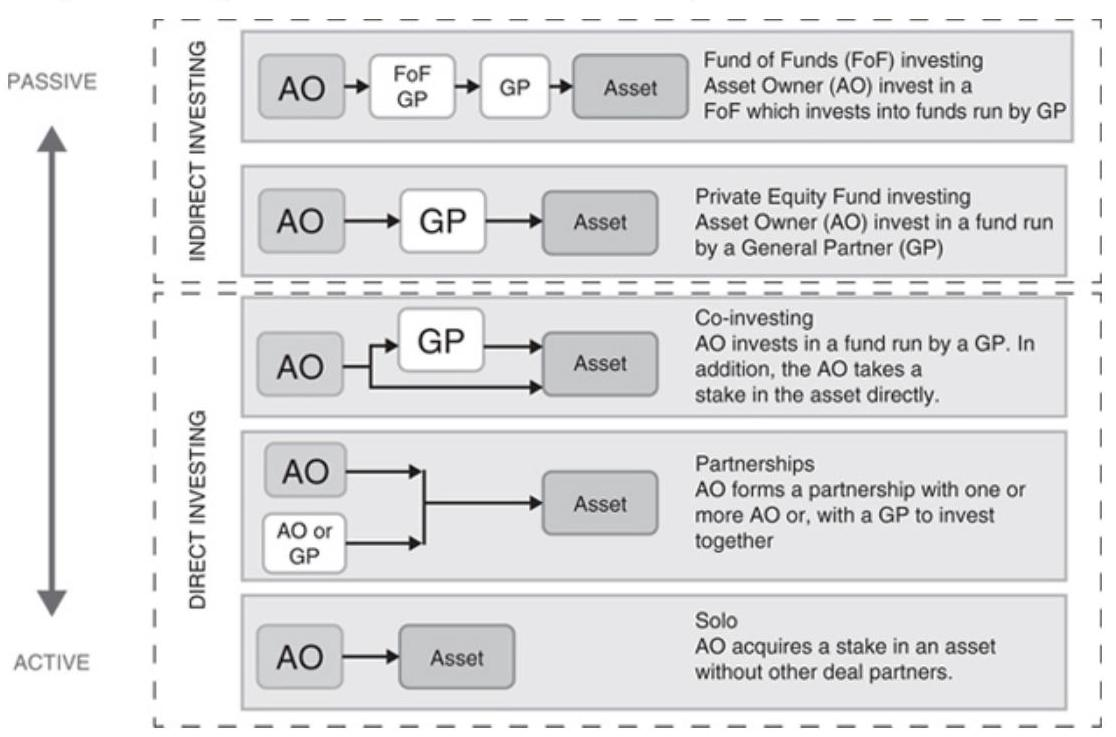
\includegraphics[max width=\textwidth]{2024_04_10_b9f91501c03ad990a1d8g-2}
\end{center}

Methods of Direct and Indirect Private Equity Investment Source: CAIA Association

When asset owners get more sophisticated and experienced in investing in PE, they may consider direct investing. There are three main models of direct investing:

\begin{itemize}
  \item Solo investing represents direct investing without any other deal partners; thus it requires the most active management from the asset owner. With solo direct investing, an asset owner not only makes the investment decision, but also sources the investments and performs-or directly oversees-critical investment activities, including due diligence and ongoing asset management.
  \item Partnership investing involves an asset owner forming a partnership with one or more asset owners or, sometimes, with a GP, to invest together in a specific deal or a series of deals over time. The partnership approach can be attractive because it allows an asset owner to pursue larger deals, enables a broader range of deal sourcing, and can help mitigate risk. For example, a foreign investor can benefit from a partnership with a local investor who has on-the-ground knowledge and relationships.
  \item Co-investment refers to the practice of asset owners being invited by the sponsors of private equity funds (typically GPs) to make investments into one or more prespecified portfolio companies using structures other than a main private equity fund. Co-investment is somewhat of a middle ground between direct and fund investment. Typically, in co-investment, an asset owner makes an investment alongside an existing GP with whom they already have a fund investment. Since fees are generally reduced on co-investments, asset owners making co-investments can leverage the skills of the GP, increase their allocation to PE, and pay lower aggregate fees.
\end{itemize}

\section*{What Drives Direct Investments?}
Asset owners pursue direct investments for three key reasons:

\begin{itemize}
  \item Improve returns while managing risk. Direct investing allows asset owners to tailor their portfolios more specifically to their needs and take advantage of their long-term horizon. It allows asset owners to invest in assets that may not fit into the traditional fund construct. For example, if an asset owner wants to hold an asset for decades, or indefinitely, it would be more suitable for the asset owner to invest directly into the portfolio company instead of through a traditional fund structure. For the experienced asset owner with broad set of relationships, direct investing provides the opportunity to leverage those relationships to select the best assets with attractive risk profiles and find ways to deploy capital with lower competition.
  \item Control. Direct investing provides an asset owner with more control over its portfolio, as the asset owner is not reliant on the GP on when to sell an asset. It also allows the asset owner to avoid investing alongside asset owners who do not share a similar investment time horizon or liquidity profile. During the global financial crisis of 2007-2009, many asset owners found they lacked control over their investments when fellow LPs had liquidity challenges that led them to sell\\
their stakes or seek redemptions in the fund. Furthermore, some asset owners may find it difficult to obtain information from GPs about the underlying portfolio companies during that period. Direct investment gives the asset owner greater control of underlying investments and greater information flow.
  \item Cost efficiency. Many asset owners are keen to manage costs effectively while capturing alpha in order to achieve a higher expected return. For asset owners with certain scale and sophistication, they could build an in-house team to manage a direct investment program for similar or lower costs than those incurred when using external managers. The costs of running a direct-investing program can vary significantly, depending on the model adopted and the type of assets. Typically, a solo investing approach is more expensive to set up and run than partnership investing, which is more expensive than co-investing. Direct investment removes the intermediaries between the asset owner and the underlying assets, which could reduce the operational complexities and costs.
\end{itemize}

\section*{What Is the Most Common Type of Direct Investments?}
While direct investing is gaining popularity amongst asset owners, data show that asset owners have increased their co-investment activities but not solo investment activities. A 2017 Coller Capital Survey ${ }^{1}$ Coller Capital 2017 Survey, Global Private Equity Barometer. Page 8. Figure 16 and Figure 17, \href{https://www.collercapital.com/sites/default/files/Coller%20Capital%20Global%20Private%20Equity%20Barometer%20Winter%202017-18.pdf}{https://www.collercapital.com/sites/default/files/Coller Capital Global Private Equity Barometer Winter 2017-18.pdf} noted that the proportion of investors making co-investments in private equity grew from $42 \%$ in 2012 to $55 \%$ in 2018, while the proportion of investors making solo investments only grew from $30 \%$ in to $31 \%$ over the same period.

The exhibit Among Direct Strategies, Co-Investment Has Increased Significantly shows the trend of co-investment and direct investment, highlighting the fact that coinvestment has increased significantly. Co-investment activities are also linked to PE fundraising. Some industry experts estimate that for every dollar raised by GPs, an additional 20 cents is deployed in global co-investment opportunities. ${ }^{2}$ Hamilton Lane (2019), Co-investing: The Struggle Is Real.

\begin{center}
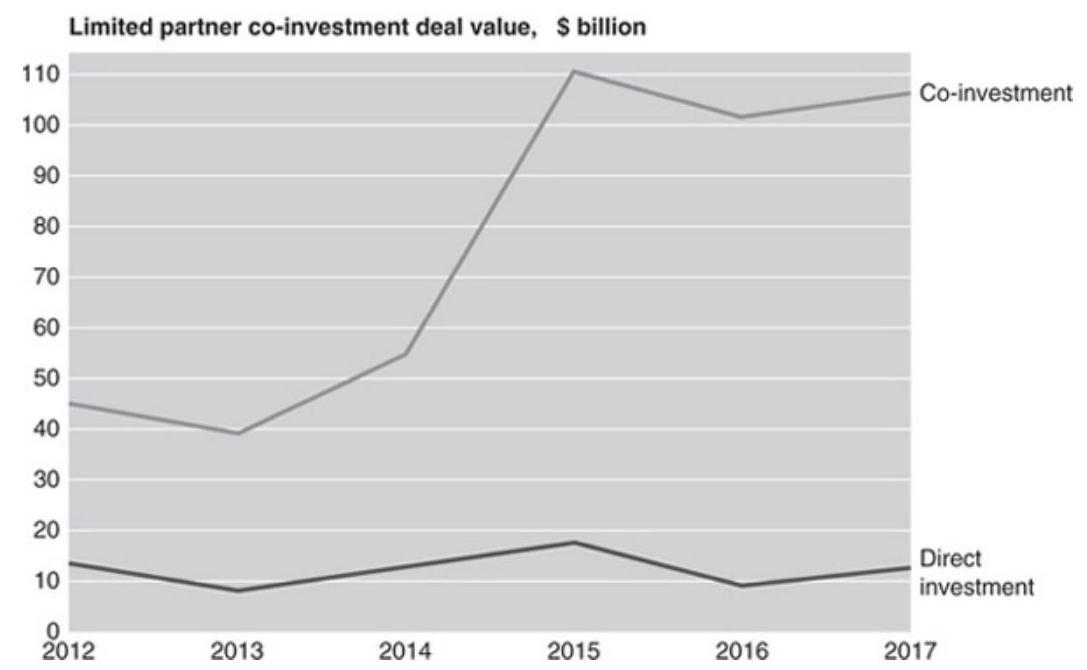
\includegraphics[max width=\textwidth]{2024_04_10_b9f91501c03ad990a1d8g-3}
\end{center}

Among Direct Strategies, Co-Investment Has Increased Significantly

Source: Exhibit from "The rise and rise of private markets, McKinsey Global Private Market Review”, February 2018, McKinsey \& Company, \href{http://www.mckinsey.com}{www.mckinsey.com}. Copyright (c) 2021 McKinsey \& Company. All rights reserved. Reprinted by permission.


\end{document}